%==============================Kapitola: Speciální teorie relativity=================================
\chapter{Speciální teorie relativity}
\minitoc
\newpage
  \section{Princip relativity}
    Více než 200 let se věřilo, že Newtonovy ronice správně popisují přírodu. Když se v nich poprvé 
    našla chyba, našel se i způsob, jak jej odstranit. Oboje, chybu i korekci, objevil Einstein v 
    roce 1905.
    
    V druhém Newtonově zákoně, daném vztahem $$\vr{F} = \der{(mv)}{t}$$ se mlčky předpokládalo, že 
    $m$ je konstantní veličina. Ale nyní víme, že to není pravda a že hmotnost tělesa roste, 
    zvyšuje-li se jeho rychlost. V Einsteinově opraveném vztahu má $m$ hodnotu 
    \begin{equation}\label{TEMP:eq_fey_rel_01}
      m = \frac{m_0}{\sqrt{1-\frac{v^2}{c^2}}}
    \end{equation}  
    kde $m_0$ je \emph{klidová hmotnost} (hmotnost tělesa, jež se nepohybuje) a $c$ je 
    \emph{rychlost světla}, která je přibližně rovna $3\cdot10^5\,
    km\cdot s^{-1}$.
    
    Ze vztahu je vidět, že za normálních okolností je přírůstek hmotnosti velmi malý. Dokonce i pro 
    družici Země, jež se pohybuje rychlostí $9,0\, km\cdot s^{-1}$ je $v/c = 3\cdot10^{-5}$ a po 
    dosazení do uvedeného vztahu dostaneme korekci hmotnosti ne větší než dvě až tři miliardtiny, 
    což téměř nelze pozorovat. Platnost vztahu však byla dostatečně potvrzena pozorováním mnoha 
    druhů částic, jejichž rychlosti dosahují prakticky až rychlosti světla. Za normálních okolností 
    je tento efekt velmi malý a proto je pozoruhodné, že byl objeven nejprve teoreticky a až potom 
    experimentálně. Proto je zajímavé sledovat, jaké kombinace experimentů a fyzikálních úvah vedla 
    k odhalení tak jemné modifikace zákona. Přispělo k tomu nemálo lidí, přičemž konečným výsledkem 
    byl Einsteinův objev.
    
    Existují dvě Einsteinovy teorie relativity. Tato kapitola hovoří o \emph{speciální teorii 
    relativity} z roku 1905. V roce 1915 uveřejnil Einstein dodatečnou teorii nazvanou \emph{Obecná 
    teorie relativity}. Ta je zobecněním speciální teorie relativity pro případ \emph{gravitace}.
         
    Newton byl první, kdo vyslovil \emph{princip relativity} jako jeden z důsledků pohybových 
    zákonů: Vzájemné pohyby těles, nacházejících se v daném prostoru, jsou stejné ať je prostor v 
    klidu, nebo se pohybuje rovnoměrně přímočaře vpřed. To například znamená, že jestliže se 
    kosmická loď pohybuje rovnoměrnou rychlostí, všechny experimenty a všechny jevy v lodi budou 
    probíhat tak, jakoby se loď nepohybovala (samozřejmě za předpokladu, že se nikdo nebude dívat 
    ven). To je smyslem principu relativity. Myšlenka je jednoduchá, jedinou otázkou je, zda je 
    pravda, že ve všech experimentech provedených v pohybující se soustavě budou všechny fyzikální 
    zákony stejné, jako v soustavě, která je v klidu. Nejprve zjistíme, zda v pohybující se soustavě 
    mají Newtonovy zákony stejný tvar.        
    
    \begin{figure}
      \centering
      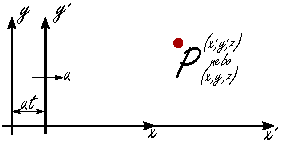
\includegraphics[width=0.8\linewidth]{fey_princip_relativity.pdf}
      \caption{Dvě souřadnicové soustavy v rovnoměrném relativním pohybu podél svých x-ových os.}
      \label{fyz:fig_fey_spec_relativita}
    \end{figure}
    
    Předpokládejme, že se Pavel pohybuje konstantní rychlostí $u$ ve směru osy $x$, přičemž měří 
    polohu určitého budu (obr. \ref{fyz:fig_fey_spec_relativita}). Ve své souřadnicové soustavě si 
    značí souřadnici ve směru osy $x$ jako $x'$. Petr je v klidu, přičemž měří polohu téhož bodu. 
    Souřadnici ve směru osy $x$ ve své souřadnicové soustavě značí jako $x$. Počátek souřadnicové 
    soustavy, v níž je Pavel, se posunu za čas $t$ o vzdálenost $ut$, a jestliže soustavy z počátku 
    splývaly, máme
    \begin{equation}\label{TEMP:eq_fey_rel_02}
      x' = x - ut, \qquad y' = y, \qquad z' = z, \qquad t' = t. 
    \end{equation}      
    Dosadíme-li tuto transformaci do Newtonových zákonů, zjistíme, že se přetransformovaly do 
    stejných zákonů v čárkované soustavě. To znamená, že Newtonovy zákony mají stejný tvar v 
    pohybující se soustavě jako v stacionární soustavě, a proto na základě mechanických experimentů 
    není možné říci, zda se soustava pohybuje či nikoliv. 
    
    Zájem o tento princip vzrostl v minulém století v důsledku výzkumu elektrických, magnetických a 
    světelných jevů, jež vyústilo v \emph{Maxwellovu teorii elektromagnetického pole}, která 
    jednotně popisuje elektřinu, magnetizmus a světlo. Zdálo se však, že Maxwellovy rovnice 
    nevyhovovaly \emph{principu relativity}, neboť přetransformujeme-li Maxwellovy rovnice pomocí 
    rovnic \ref{TEMP:eq_fey_rel_02}, nebudou mít stejný tvar. Proto by se elektrické a optické jevy 
    v letící kosmické lodi měli lišit od jevů v nehybné lodi. Těmito jevy by pak bylo možné určit 
    rychlost lodi, a ve speciálním případě pomocí vhodných optických nebo elektrických měření by 
    bylo možné určit i absolutní rychlost lodi. Jedním z důsledků Maxwellových rovnic je, že 
    dojde-li k určité poruše pole, při níž vniká světlo, toto elektromagnetické vlnění se šíří všemi 
    směry stejnou rychlostí $c = 3\cdot10^5\,km\cdot s^{-1}$. Dalším důsledkem těchto rovnic je, že 
    pohybuje-li se zdroj poruchy, šíří se vyzářené světlo prostorem stejnou rychlostí $c$. Tato 
    nezávislost pohybu vlnění na pohybu zdroje vede k zajímavému problému:
    
    Předpokládejme, že sedíme v autě, jež jede rychlostí $u$ a že světlo z reflektorů auta za námi 
    nás míjí rychlostí $c$. Zdiferencováním první rovnice \ref{TEMP:eq_fey_rel_02} máme
    \begin{equation}\label{TEMP:eq_fey_rel_03}
      \der{x'}{t} =\der{x}{t} - u, 
    \end{equation}       
    což znamená, že podle \emph{Galileovy transformace} by zdánlivá rychlost světla měřená z auta 
    nemohla být $c$, ale $c-u$. Na této myšlence bylo založeno mnoho experimentů k určení rychlosti 
    Země, ale všechny selhaly - nedávaly vůbec žádné rychlosti. Ukázalo se, že někde byla chyba, a 
    sice něco nebylo v pořádku s fyzikálními rovnicemi. Co to asi mohlo být?

  %------------------------ Lorentzova transformace -------------------------------------------------
  \section{Lorentzova transformace}
    Když se zjistilo, že s rovnicemi v uvedeném případě není vše v pořádku, nejprve padlo podezření 
    na Maxwellovy rovnice elektrodynamiky, jež byly tehdy známy jen dvacet let. Zdálo se být téměř 
    samozřejmé, že tyto rovnice musí byt nesprávné a proto byla snaha je změnit tak, aby při 
    Galileiho transformaci zachovávaly princip relativity. Přitom bylo třeba do těchto rovnic zavést 
    nové členy, jež vedly k předpovědi nových elektrických jevů, jejichž existence se experimentálně 
    nepotvrdila. Proto bylo třeba tuto cestu opustit. Postupně se pak stalo zřejmým, že Maxwellovy 
    zákony elektrodynamiky jsou správné a zdroj problému je třeba hledat někde jinde.  
    
    Mezitím si \emph{H. A. Lorentz} všiml pozoruhodné věci, když použil v Maxwellových rovnicích substituci
    \begin{equation}\label{TEMP:eq_fey_rel_04}
      x' = \frac{x - ut}{\sqrt{1-\frac{u^2}{c^2}}}, 
           \qquad y' = y, \qquad z' = z, 
           \qquad t' = \frac{t-\frac{u}{c^2}x}{\sqrt{1-\frac{u^2}{c^2}}}. 
    \end{equation} 
    tvar rovnic se nezměnil. Rovnice \ref{TEMP:eq_fey_rel_04} jsou známé jako \emph{Lorentzovy 
    transformace}. Einstein sledoval původní Poincarého myšlenku a pak navrhl, že všechny fyzikální 
    zákony, by měly být takové, aby se při Lorentzově transformaci neměnily. Jinými slovy, měly 
    bychom změnit ne zákony elektrodynamiky, ale zákony mechaniky. Jak se ukázalo jediné co je 
    třeba, je změnit hmotnost $m$ v Newtonových rovnicích podle vztahu \ref{TEMP:eq_fey_rel_01}. Po 
    této změně budou Newtonovy zákony v souladu se zákony elektrodynamiky. Když k porovnání 
    Pavlových a Petrových měření použijeme Lorentzovu transformaci, nikdy nebudeme schopni zjistit, 
    zda se jeden nebo druhý pohybuje, neboť tvary všech rovnic budou v obou souřadnicových 
    soustavách stejné. 
    
    Pro pochopení smyslu této nové transformace nestačí studovat jen zákony mechaniky, ale podobně 
    jako Einstein, musíme provést analýzu našeho chápání prostoru a času. 

\printbibliography[heading=subbibliography]